\section{Descripción General}
En este documento se desarrollarán las motivaciones, implicaciones y detalles de la implementación de este Trabajo de Fin de Grado.

El objetivo general de este proyecto ha sido el desarrollo de un paquete de herramientas y sistemas modulares que permitan agilizar el proceso de desarrollo de un videojuego. 
El paquete está compuesto de cinco módulos distintos, que a su vez se componen de una serie de herramientas o sistemas con diversas funciones, también incluye una serie de 
escenas de prueba en las que se pueden ver los diversos sistemas en acción. Además, cada módulo y submódulo incluye todos los 'prefabs' necesarios para su funcionamiento 
inmediato. 

Los distintos módulos son: 
\begin{compactitem}
  \item Sistemas Atómicos.   
  \item Herramientas de Debug
  \item Generador de Mazmorras
  \item Componentes Independientes de Unity
  \item Componentes de Movimiento de Personajes
\end{compactitem} 
\subsection{Sistemas Atómicos}
El módulo de Sistemas Atómicos está compuesto por los siguientes submódulos:
\begin{itemize}
  \item Sistema de Diálogos: Incluye un editor de diálogos basado en grafos que permite esquematizar flujos conversacionales con distintas respuestas posibles, 
  además de exportarlo a un formato legible por otra herramienta de editor que permite colocar dichos diálogos en el nivel, con distintos tipos de desencadenantes. Además, 
  el sistema incluye una implementación de efectos de texto modular que permite añadir animaciones al texto basándose en los vértices del mallado. 
  \item Sistema de Experiencia: Es un sencillo sistema que permite definir una serie de constantes para personalizar un sistema de niveles para habilidades o personajes,
   además de poder elegir entre una serie de algoritmos para definir la curva de adquisición de experiencia. 
  \item Sistema de audio: Permite la definición de distintas canciones y sonidos como Scriptable Objects y reproducirlos en distintos canales de audio 
   mediante la invocación de funciones estáticas.
  \item Sistema de guardado: Trae una serie de funciones utilitarias que permite guardar cualquier variable alfanumérica, lista o mapa en formato JSON en el directorio 
   especificado, además de permitir encriptar dicho fichero. Este sistema trae también una implementación para varias ranuras de guardado, funciones para crear, copiar y
   eliminar ranuras de guardado.
  \item Sistema de Gestión de Carga de Escenas: Un paquete que se compone de distintas funciones que permiten cargar escenas de forma asíncrona, descargando automáticamente 
   la escena actual y permitiendo definir una pantalla de carga intermedia para hacer la transición más agradable.
\end{itemize}

\subsection{Herramientas de Debug}
Las herramientas de debug son sencillos scripts que tienen como objetivo hacer que la depuración de errores sea más cómoda, este paquete incluye:
\begin{compactitem}
  \item Componente de Dibujado de Colisiones 2D: Consiste en un componente que dibuja las colisiones en la ventana de 'play' de Unity y en versiones empaquetadas.   
  \item Herramienta de cuadrícula : Consiste en un componente que se ejecuta solo en modo debug, y hace más sencillo colocar los elementos de la escena siguiendo una
   cuadrícula de un tamaño especificado en el inspector del componente. 
\end{compactitem} 

\subsection{Generador de Mazmorras}
El generador de Mazmorras es una herramienta que utiliza una serie de algoritmos de recorrido de grafos para generar laberintos o mazmorras, e incluye una serie de clases
 utilitarias que permiten buscar el camino mínimo, convertir las estructuras de mazmorras/laberintos a grafos pesados o matrices.

\subsection{Componentes Independientes de Unity}
Este módulo contiene las características que son o bien una colección de funciones estáticas, sistemas simples contenidos en una sola clase o componentes de Unity 
 con funcionalidades sencillas.
\begin{compactitem}
  \item 'Floater': Sencillo script que hace que cualquier objeto de la escena flote siguiendo una función sinuidal. También hace que rote sobre sí mismo dada una velocidad.
  \item Componente de Vida: Permite asignar vida a un objeto y definir eventos que provocan una pérdida de vida o que reaccionen a ello. 
  \item Componente de Interacción: Permite añadir a un objeto una serie de eventos que se ejecuten cuando el jugador interactúe con el mismo. También permite definir un
   rango en el cual pueda interactuar. 
  \item 'LaunchRigidbody': Función estática que permite lanzar cualquier objeto con físicas con una dirección y fuerza específicas.
  \item 'LookAtCamera': Componente que provoca que el objeto que lo contenga siempre mire hacia cámara, útil para textos u objetos 2D de la escena.
  \item Componentes de Sacudida de Cámara: Sistema que, mediante funciones estáticas, permite sacudir cámaras de Unity o 'Cinemachine' en escenarios 2D y 3D, permite
   definir la intensidad de la sacudida basada en curvas de animación.
\end{compactitem}

\subsection{Componentes de Movimiento de Personajes}
Este módulo está compuesto por una colección de 'prefabs' que, con sus scripts asociados, permiten añadir a una escena un personaje jugable con unos controles y cámara asociados.
Todas las configuraciones posibles contienen tanto una implementación basada en movimiento discreto como otra basada en físicas, las diferentes configuraciones son: 
\begin{compactitem}
  \item 2D Lateral o 'Side Scroll': Permite jugar con un esquema de controles similar al de un plataformas clásico como 'Super Mario World' (Figura \ref{fig:smbw}).
  \item 2D Cenital o 'Top Down': Permite jugar con un esquema de controles similar al de el primer 'The Legend of Zelda' o 'Hotline Miami' (Figura \ref{fig:hlmiami}).
  \item 3D Primera Persona o 'First Person': Permite jugar con un esquema de controles similar a 'Doom' o 'Call of Duty' (Figura \ref{fig:doometernal}).
  \item 3D Tercera Persona o 'Third Person': Permite jugar con un esquema de controles similar a 'Grand Theft Auto', 'God of War: Ragnarok' o 'Blades of Fire' (Figura \ref{fig:bof}). Esta configuración permite escoger entre varios 
   tipos de posicionamiento de cámara para ese mismo esquema, como por ejemplo: tercera persona clásica , vista cenital, isométrica, o cámara al hombro. 
  \item 3D Lateral o 'Side Scroll': Permite jugar con un esquema de controles similar a 'Metroid Dread' (Figura \ref{fig:mdread}).
\end{compactitem}
\raggedbottom
\begin{figure}[H]
  \centering
    
\includegraphics[width=350px,clip=true]{super_mario_world.jpg}
  \caption{2D side scroll, Super Mario World.}
  \label{fig:smbw}
\end{figure}

\begin{figure}[H]
  \centering
  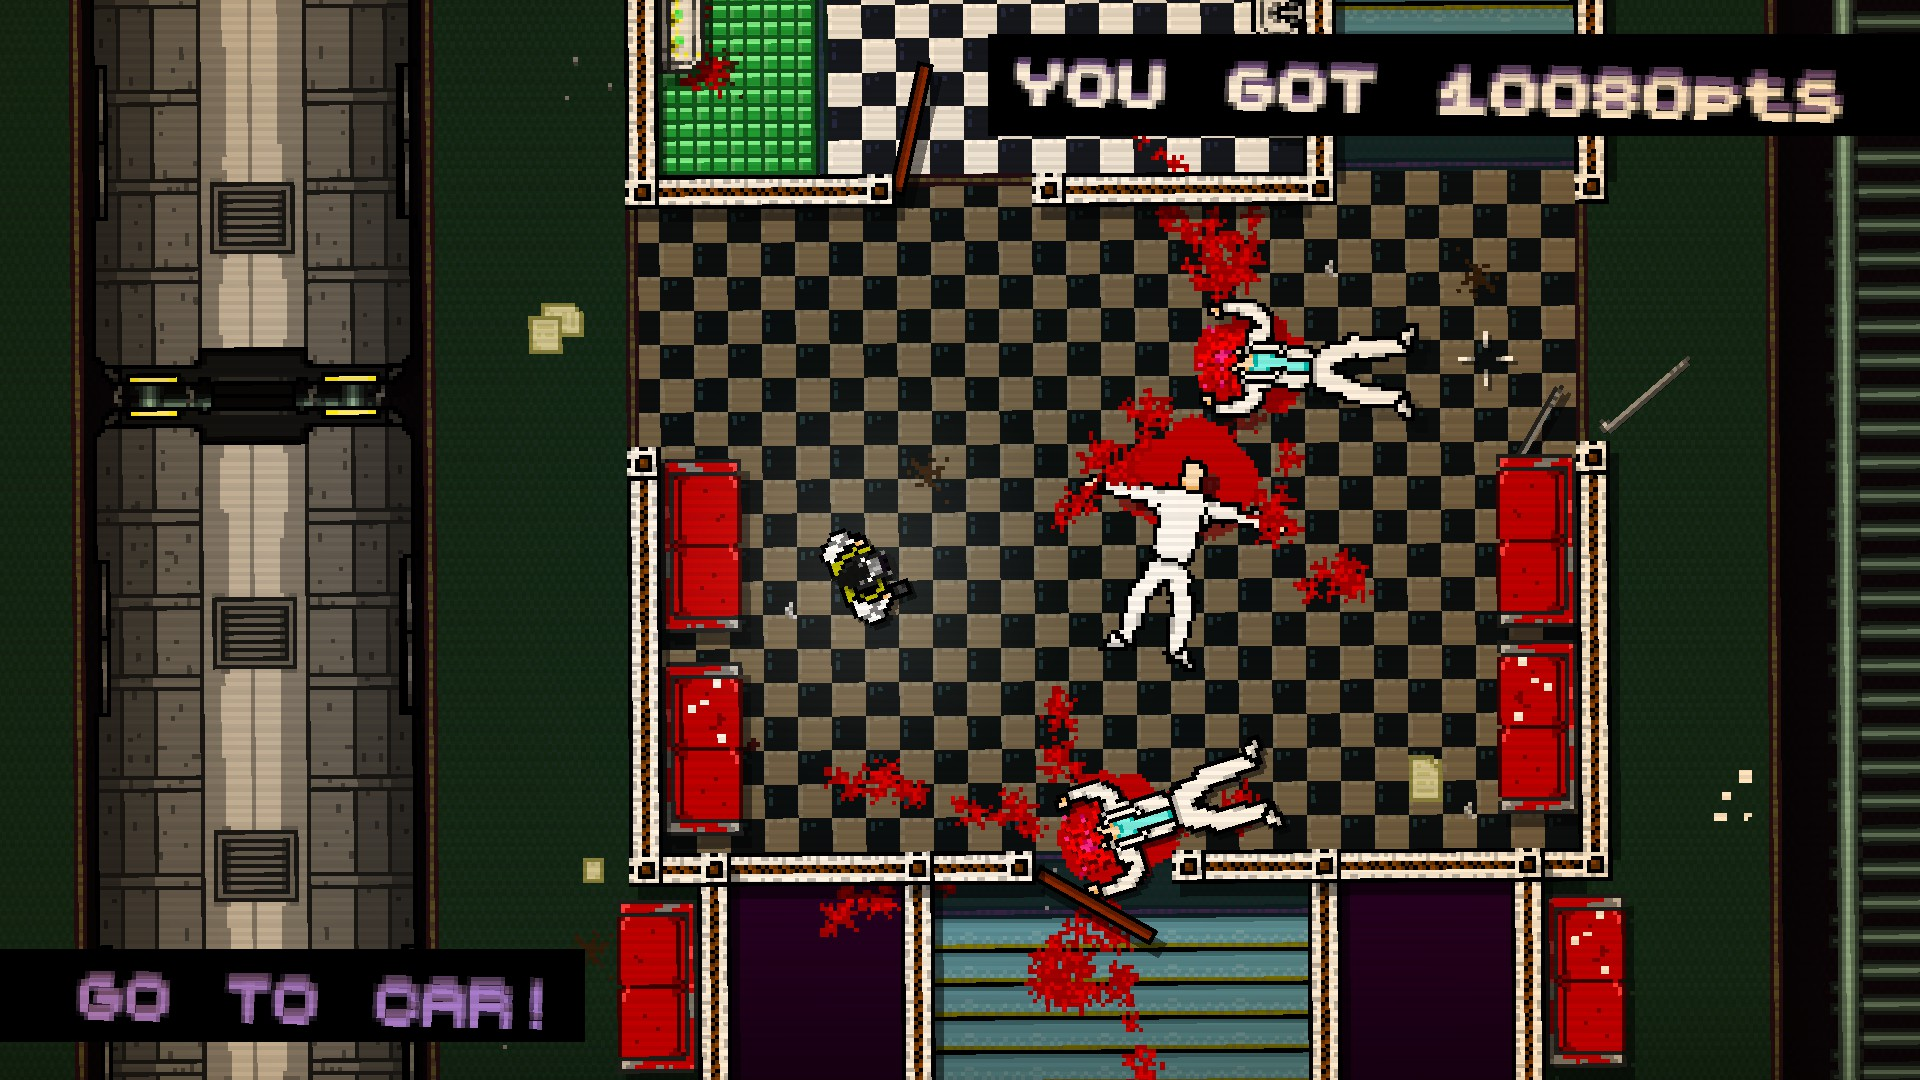
\includegraphics[width=350px,clip=true]{hotline_miami.png}
  \caption{2D top down, Hotline Miami.}
  \label{fig:hlmiami}
\end{figure}

\begin{figure}[H]
  \centering
  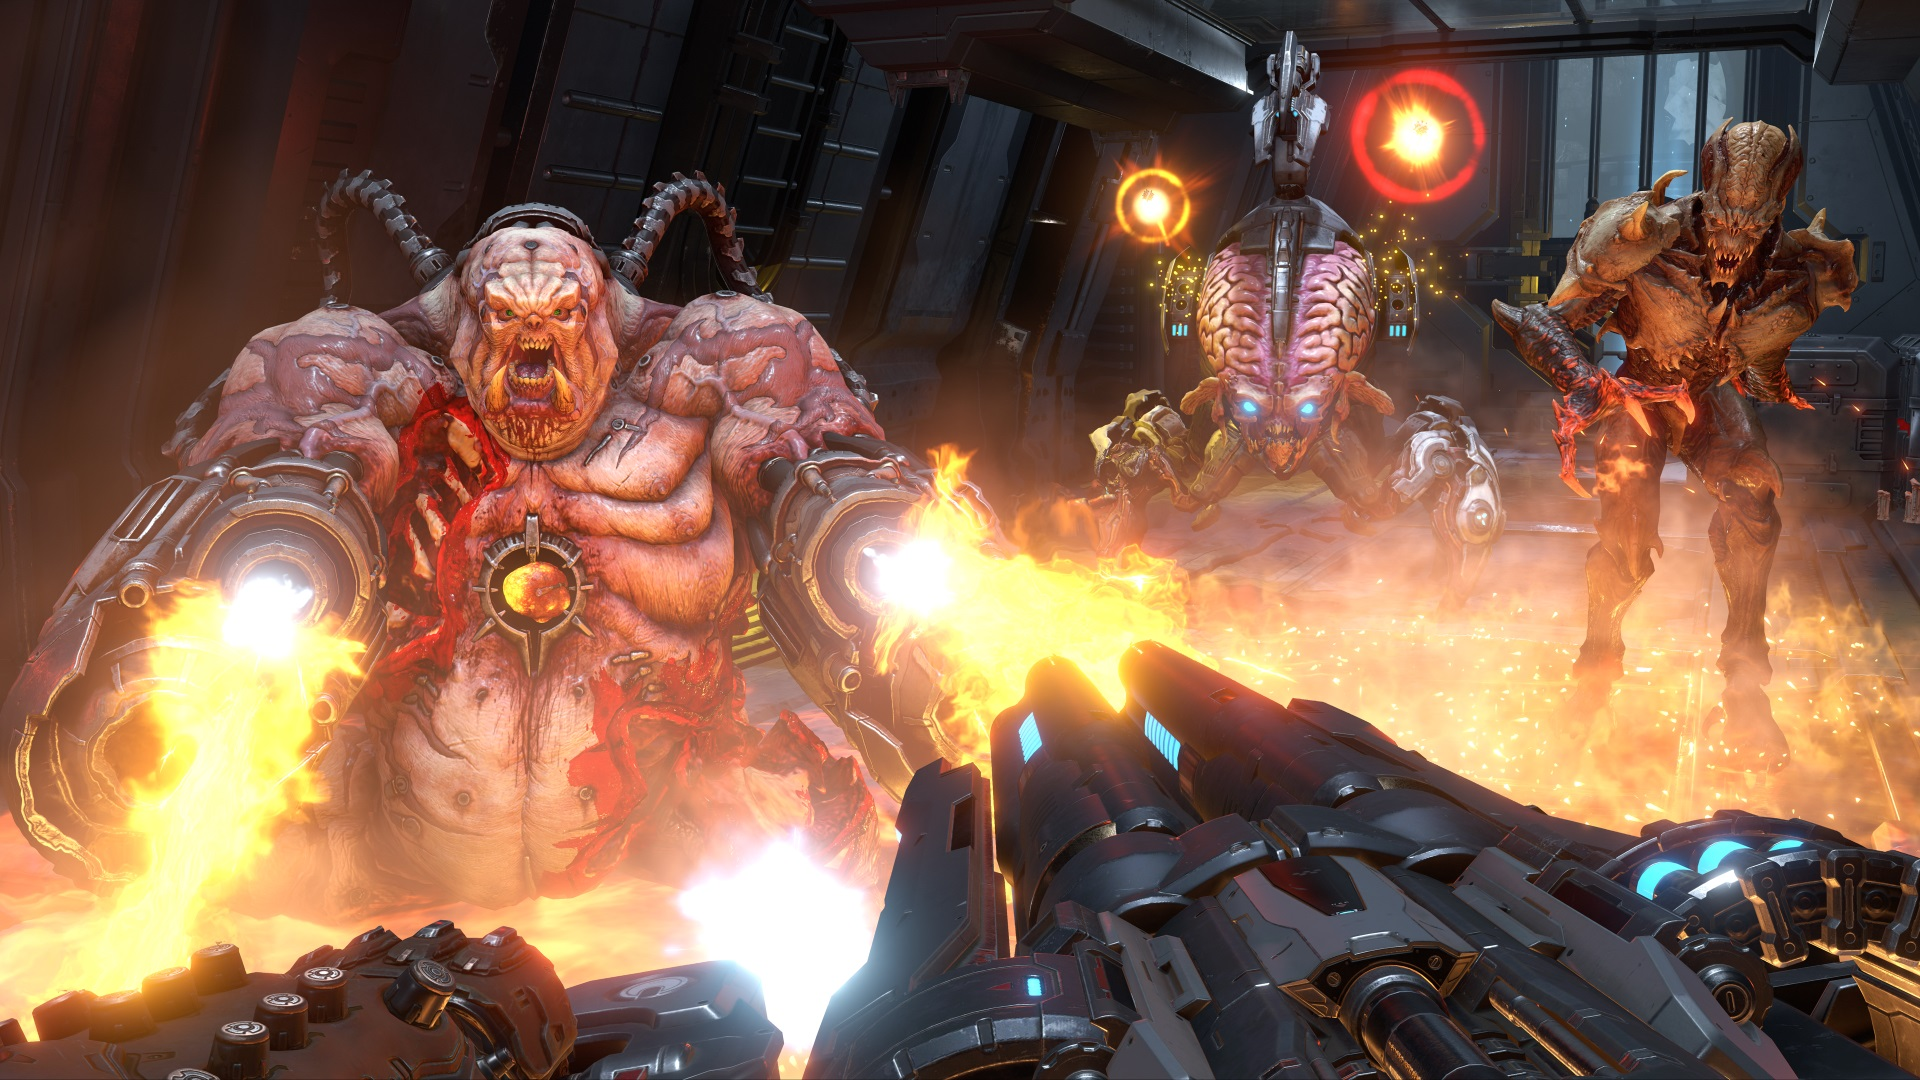
\includegraphics[width=350px,clip=true]{doom_eternal.png}
  \caption{3D primera persona, Doom Eternal.}
  \label{fig:doometernal}
\end{figure}

\begin{figure}[H]
  \centering
  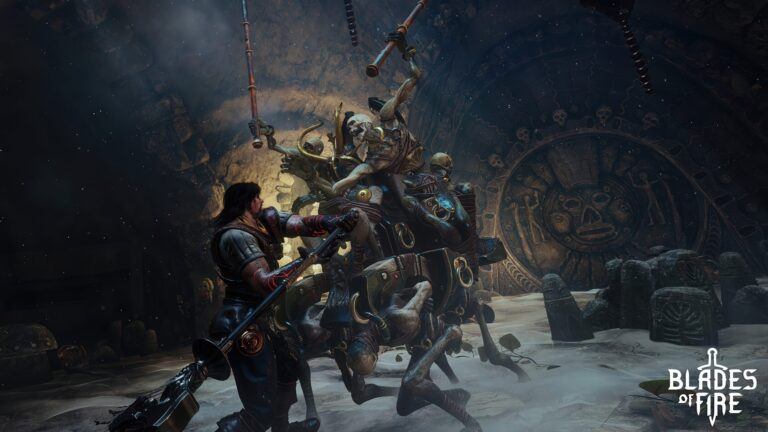
\includegraphics[width=350px,clip=true]{bof.png}
  \caption{3D tercera persona, Blades of Fire.}
  \label{fig:bof}
\end{figure}

\begin{figure}[H]
  \centering
  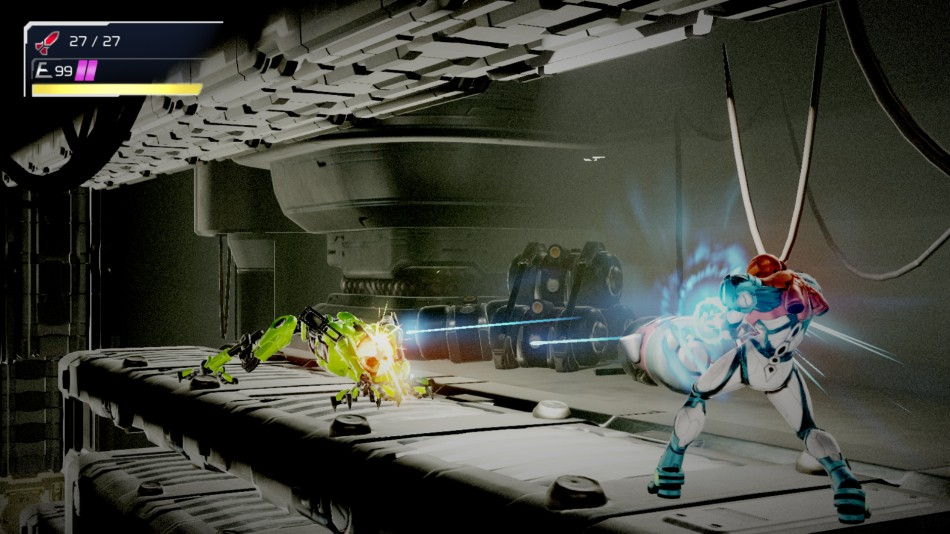
\includegraphics[width=350px,clip=true]{dread.png}
  \caption{3D side scroll, Metroid Dread.}
  \label{fig:mdread}
\end{figure}

\section{Motivación}

La motivación para el desarrollo de este proyecto ha sido la reiterada necesidad de una serie de funcionalidades básicas a lo largo de mi trayectoria como desarrollador,
 en trabajos de clase, participando en 'Game Jams' o en proyectos independientes. Pese a que algunas de las funcionalidades contenidas en el paquete ya existen en el mercado,
 se ha buscado en todos los casos aportar una solución más general, funcional y escalable que las alternativas disponibles. El resultado es un paquete que intenta proporcionar
 una 'suite' de herramientas que agilicen el prototipado de videojuegos, y permitan ampliar la funcionalidad base conforme el proyecto requiera de funciones más específicas. 
 Por tanto se puede extraer que tanto una motivación como un objetivo sería desarrollar una librería de funcionalidades que pueda asistir a equipos futuros a desarrollar
 videojuegos de forma más ágil.

Este enfoque tiene como objetivo que el paquete sea lo más transversal y usable posible para desarrolladores de todos los niveles (siempre y cuando tengan una formación básica).
 De forma que permite a desarrolladores sin mucha experiencia utilizar el paquete en su forma básica, la cual contiene suficiente funcionalidad como para poder crear juegos
 sencillos, además de permitir a desarrolladores más experimentados utilizar y evolucionar las herramientas para crear mecánicas y dinámicas complejas.
 
 Finalmente habría que considerar también la motivación adicional de aprender el uso de nuevas tecnologías mediante el desarrollo de un proyecto, que tendría como objetivo el
  propio aprendizaje y la acumulación de experiencia de llevar un proyecto desde su etapa de concepción hasta validarlo con el prototipado y finalización de un videojuego. 

%\raggedbottom
\section{Objetivos}
\subsection{Objetivos generales}
El objetivo general del trabajo es la elaboración de una librería completa y funcional con la los usuarios puedan prototipar videojuegos de forma ágil y sencilla. 
 En dicha librería deberían haber sistemas que permitan gestionar diálogos, archivos de guardado, sonido, niveles y cargas. Además de componentes independientes que permitan 
 el uso de físicas, movimiento y sacudida de cámara. Además, deberá incluir herramientas de depuración propias para auxiliar tanto las herramientas propias como las del motor. 
 Finalmente la 'suite' de herramientas deberá permitir la generación procedimental de laberintos y mazmorras.

\subsection{Escalabilidad}
El objetivo más importante del proyecto, por encima de implementar todas las características deseadas, es que todos los componentes queden bien documentados, sean funcionales
 y escalables. De forma que, como se ha mencionado anteriormente, usuarios con cualquier nivel de experiencia puedan hacer uso de las herramientas expuestas. De este modo, 
 además de pulir dichas herramientas, el código debe de estar implementado de forma que, ya sea mediante patrones, composición y/o herencia, se pueda ampliar la funcionalidad dispuesta
 cómodamente.
 
\subsection{Documentación}
Como consecuencia, para mantener un código limpio y escalable, es necesario escribir un documento detallando el modo de uso y funcionamiento de todas las características del paquete.

\subsection{Niveles de prueba}
Otro de los objetivos es construir niveles de prueba que puedan servir a los usuarios como tutoriales o ejemplos del uso de las herramientas incluidas en el paquete. Dichos 
 niveles deben estar bien organizados y etiquetados, y deben permitir a los usuarios entender como funcionan los componentes que habiten en ellos.

\subsection{Validación}

El paquete necesitará ser validado por usuarios reales, que utilicen las herramientas proporcionadas por el mismo para desarrollar un prototipo jugable, para conseguir esto,
 se prepararán al menos dos equipos que participarán en una 'Game Jam' y desarrollarán dicho prototipo disponiendo de las herramientas de la librería que crean convenientes.
 Al finalizar el evento, estos usuarios deberán rellenar una encuesta de satisfacción acerca de la librería, y se llevarán a cabo los ajustes que se puedan extrapolar de
 los resultados.  

\subsection{Resumen de Objetivos}

En resumen, el el proyecto pretende, como objetivo principal desarrollar un paquete de herramientas completo y funcional que permita a los usuarios prototipar y 
 desarrollar videojuegos. Dicho paquete debe contener diversos sistemas y componentes 'prefabricados' que agilicen el desarrollo. 

Además de los objetivos secundarios:
\begin{compactitem}
  \item Que los componentes del paquete sean escalables.
  \item Desarrollar niveles de prueba para servir a modo de tutorial para los usuarios.
  \item Documentar el modo de uso y funcionamiento de los componentes del proyecto.
  \item Validar el paquete con usuarios reales.
  \item Construir varios prototipos utilizando el paquete.
  \item Ajustar el paquete en base a los resultados de una encuesta de satisfacción.
\end{compactitem}